\documentclass[a4paper,11pt]{article}
\usepackage[utf8]{inputenc}
\usepackage[margin=1in]{geometry}
\usepackage{pdfpages}
\usepackage{mathrsfs}
\usepackage{amsfonts}
\usepackage{amsmath}
\DeclareMathOperator\arctanh{arctanh}
\usepackage{amssymb}
\usepackage{bbm}
\usepackage{amsthm}
\usepackage{graphicx}
\usepackage{centernot}
\usepackage{caption}
\usepackage{subcaption}
\usepackage{braket}
\usepackage{pgfplots}
\usepackage{lastpage}
\usepackage{enumitem}
\usepackage{setspace}
\usepackage{xcolor}
\usepackage{cancel}
\usepackage{scrextend}
\usepackage[english]{babel} 

\usepackage[square,sort,comma,numbers]{natbib}
\usepackage[colorlinks=true,linkcolor=blue]{hyperref}

\usepackage{fancyhdr}
\newcommand{\euler}[1]{\text{e}^{#1}}
\newcommand{\Real}{\text{Re}}
\newcommand{\Imag}{\text{Im}}
\newcommand{\supp}{\text{supp}}
\newcommand{\pare}[1]{\left( #1 \right)}
\newcommand{\norm}[1]{\left\lVert #1 \right\rVert}
\newcommand{\abs}[1]{\left\lvert #1 \right\rvert}
\newcommand{\floor}[1]{\left\lfloor #1 \right\rfloor}
\newcommand{\Span}[1]{\text{span}\left(#1\right)}
\newcommand{\dom}[1]{\mathscr D\left(#1\right)}
\newcommand{\Ran}[1]{\text{Ran}\left(#1\right)}
\newcommand{\conv}[1]{\text{co}\left\{#1\right\}}
\newcommand{\Ext}[1]{\text{Ext}\left\{#1\right\}}
\newcommand{\vin}{\rotatebox[origin=c]{-90}{$\in$}}
\newcommand{\vnotin}{\rotatebox[origin=c]{-90}{$\notin$}}
\newcommand{\interior}[1]{%
	{\kern0pt#1}^{\mathrm{o}}%
}
\newcommand*\diff{\mathop{}\!\mathrm{d}}
\newcommand{\ie}{\emph{i.e.} }
\newcommand{\eg}{\emph{e.g.} }
\newcommand{\dd}{\partial }
\newcommand{\N}{\mathbb{N}}
\newcommand{\Z}{\mathbb{Z}}
\newcommand{\R}{\mathbb{R}}
\newcommand{\C}{\mathbb{C}}
\newcommand{\w}{\mathsf{w}}

\newcommand{\Gliminf}{\Gamma\text{-}\liminf}
\newcommand{\Glimsup}{\Gamma\text{-}\limsup}
\newcommand{\Glim}{\Gamma\text{-}\lim}
\newcommand{\pipe}{\ \vert \ }
\newcommand{\tm}{\text{-}}

\newtheorem{theorem}{Theorem}
\newtheorem{definition}{Definition}
\newtheorem{proposition}{Proposition}
\newtheorem{lemma}{Lemma}
\newtheorem{corollary}{Corollary}

\numberwithin{equation}{section}
\linespread{1.3}

\pagestyle{fancy}
\fancyhf{}
\rhead{CoCo - Exam 2021}
\lhead{}
\rfoot{\thepage}
\lfoot{Dated: \today}
\author{Johannes Agerskov}
\date{Dated: \today}
\title{CoCo - Exam 2021}
\begin{document}
	
	\maketitle
	\textbf{Some of the problem describtions below have been copied from the exam sheet.}
	\section*{Question 1}
	Consider the following languages over the alphabet $\Sigma=\{a, b, c\}:$
	
	$$
	\begin{array}{l}
	L_{1}=\left\{w \in \Sigma^{*}: w\right.$ contains an odd number of occurrences of the letter $\left.a\right\}\\
	L_{2}=\left\{a^{m} b^{n} c^{m+n}: m, n \in \mathbb{N}\right\} \\
	L_{3}=\left\{a^{m} c^{m+n} b^{n}: m, n \in \mathbb{N}\right\} \\
	L_{4}=\left\{a^{m} c^{m^{2} n^{2}} b^{n}: m, n \in \mathbb{N}\right\}
	\end{array}
	$$
	\subsection*{Part 1.1}
	We show that $ L_1 $ is regular, and it thus follows that it also is context-free by Corollary 2.32 in M. Sipser.
	\begin{proof}
		The DFA in Figure \ref{fig:1} recognizes $ L_1 $, it then follows from definition 1.16 that $ L_1 $ is regular.
		\begin{figure}[h!]
			\centering
			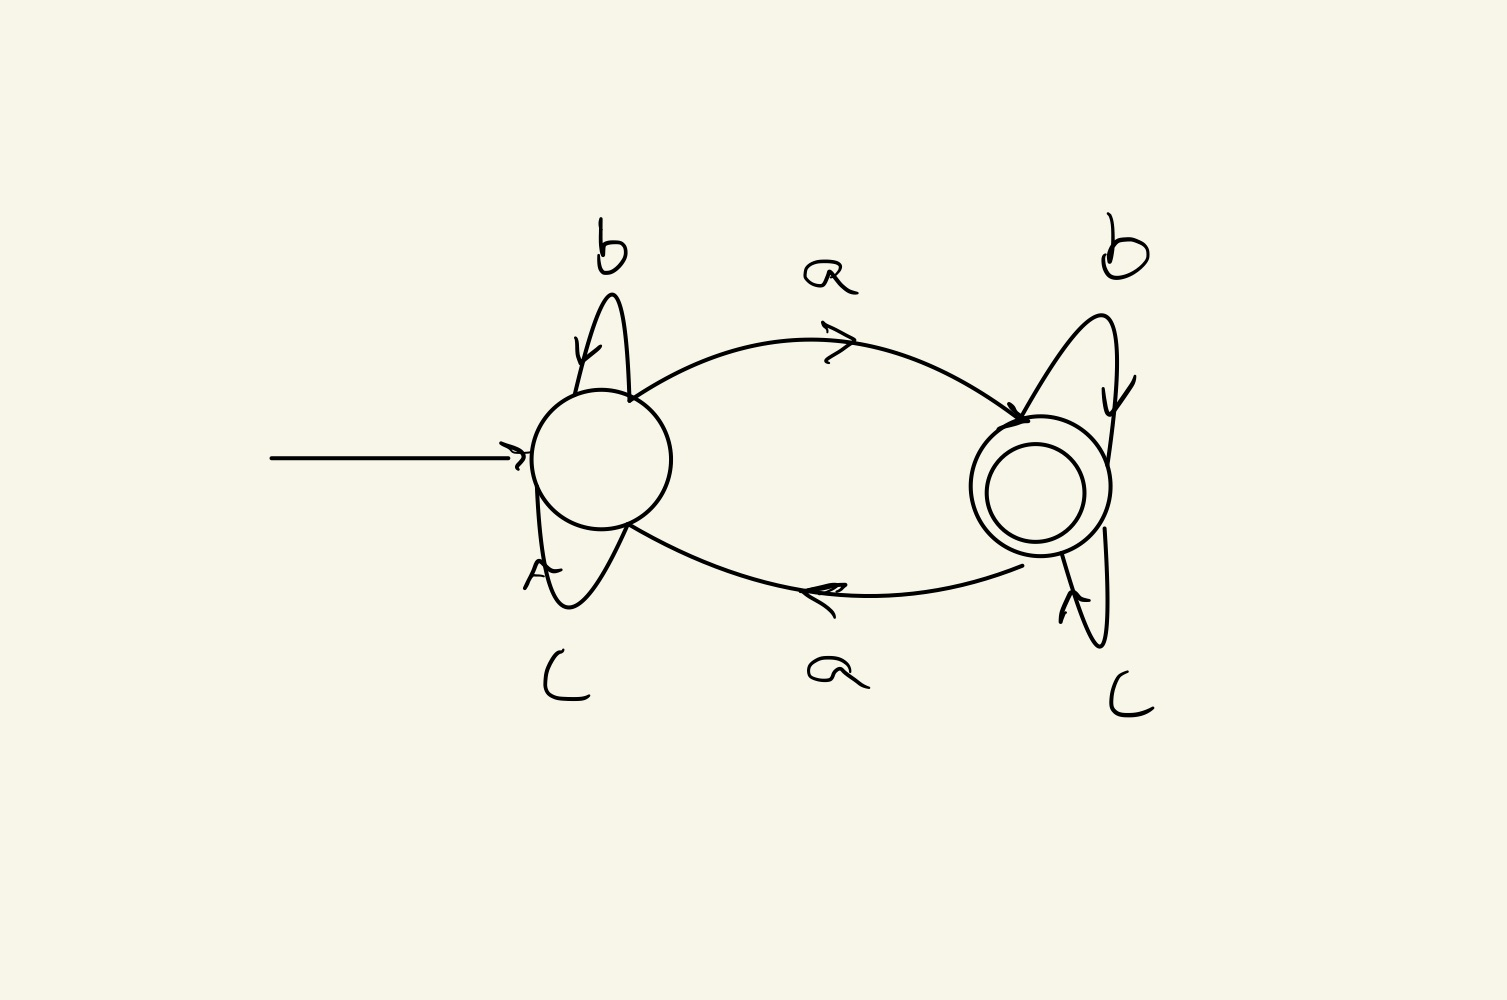
\includegraphics[width=12cm]{dfa1.jpg}
			\caption{DFA that reckognizes $ L_1$}
			\label{fig:1}
		\end{figure}
	\end{proof}
	
	\subsection*{Part 1.2}
	We show that $ L_2 $ is not regular, but it is context-free.
	\begin{proof}
		That is $ L_2 $ is not regular can be seen by the following proof by contradiction: Assume $ L_2 $ is regular, and let $ p $ denote the pumping length as given by the pumping lemma for regular languages Theorem 1.70. Consider now the string $ w=a^pb^pc^{2p}\in L_2 $, which clearly satisfies $ \abs{w}>p $. Thus by the pumping lemma we can split $ w=xyz $ with $ \abs{xy}\leq p $ and $ \abs{y}>0 $. Clearly we then have $ xy=a^k $ for some $ 0<k\leq p $, and therefore $ y=a^m $ for some $ 0<m\leq p $. But then clearly $ xy^iz=a^{p+(i-1)m}b^pc^{2p} $ which for $ i\neq 1 $ is not in $ L_2 $, contradicting the pumping lemma. Thus we conclude that $ L_2 $ is not regular. \\
		That $ L_2 $ is context-free can be seen by the fact that it is generated by the CFG\begin{equation*}
			\begin{aligned}
			S&\to aAc,\\
			A&\to aAc\pipe bBc,\\
			B&\to bBc\pipe\epsilon.
			\end{aligned}
		\end{equation*}
		Notice that it is not clear wether $ \N $ contains $ 0 $ or not. Since the concention in M. Sipser is $ \N=\{1,2,3,....\} $ that is what is used here. But even if $ \N=\{0,1,2,...\} $ $ L_2 $ is still context-free since then if is generated by CFG
		\begin{equation*}
		\begin{aligned}
		S&\to aAc\pipe\epsilon,\\
		A&\to aAc\pipe B,\\
		B&\to bBc\pipe\epsilon.
		\end{aligned}
		\end{equation*}
	\end{proof}
	
	\subsection*{Part 1.3}
	We show that $ L_3 $ is not regular, but it is context-free.
	\begin{proof}
		The proof essentially goes as that for $ L_2 $. \\
		That is $ L_3 $ is not regular can be seen by the following proof by contradiction: Assume $ L_3 $ is regular, and let $ p $ denote the pumping length as given by the pumping lemma for regular languages Theorem 1.70. Consider now the string $ w=a^pb^{2p}c^{p}\in L_3 $, which clearly satisfies $ \abs{w}>p $. Thus by the pumping lemma we can split $ w=xyz $ with $ \abs{xy}\leq p $ and $ \abs{y}>0 $. Clearly we then have $ xy=a^k $ for some $ 0<k\leq p $, and therefore $ y=a^m $ for some $ 0<m\leq p $. But then clearly $ xy^iz=a^{p+(i-1)m}b^{2p}c^{p} $ which for $ i\neq 1 $ is not in $ L_3 $, contradicting the pumping lemma. Thus we conclude that $ L_3 $ is not regular. \\
		That $ L_3 $ is context-free can be seen by the fact that it is generated by the CFG
		\begin{equation*}
		\begin{aligned}
		S&\to aAc^2Cc,\\
		A&\to aAc\pipe \epsilon,\\
		C&\to cCb\pipe\epsilon.
		\end{aligned}
		\end{equation*}
		if $ \N=\{1,2,3,...\} $ and by CFG
		\begin{equation*}
		\begin{aligned}
		S&\to AC,\\
		A&\to aAc\pipe \epsilon,\\
		C&\to cCb\pipe\epsilon.
		\end{aligned}
		\end{equation*}
		if $ \N=\{0,1,2,3,...\} $
	\end{proof}
	\subsection*{Part 1.4}
	We show that $ L_4 $ is not context-free, and it then clearly follows from Corollary 2.32 that $ L_4 $ is not regular.
	\begin{proof}
		Assume that $ L_4 $ is context-free, and let $ p $ be the pumping length as given by the pumping lemma for context-free languages Theorem 2.34. Consider then the string $ w=a^pc^{p^2+1}b $. By the pumping lemma we may split $ w=uvxyz $ where $ \abs{vy}>0 $ and $ \abs{vxy}\leq p $. Thus either $ vxy=a^k $ for some $ 0<k\leq p $ in which case $ vy=a^m $ for some $ 0<m\leq p $, but then $ uv^ixy^iz=a^{p+(i-1)m}c^{p^2+1}b $ which is not in $ L_4 $ for $ i\neq 1 $, contradicting the pumping lemma. Or $ vxy=a^kc^l $ for some $ 0<k+l\leq p $, but then $ vy=a^sc^t $ for some $  0<k+l\leq p  $ and $ uv^ixy^iz=a^{p+(i-1)s}c^{p^2+1+(i-1)t}b  $, but clearly there exist for any $ s,t $ such that $ s>0 $ an $ i\in\{0,1,2,...\} $ such that $ (p+(i-1)s)^2>p^2+1+(i-1)t $, and thus for such an $ i $, $ uv^ixy^iz $ is not in $ L_4 $ contradicting the pumping lemma and if $ s=0 $ we obviously have $ uv^ixy^iz=a^{p+(i-1)s}c^{p^2+1+(i-1)t}b \notin L_4 $ also contradicting the pumping lemma. Or we may have $ vxy=c^k $ for some $ 0<k\leq p $, in which case $ vy=c^m $ for some $ 0<m\leq p $, but then $ uv^ixy^iz=a^pc^{p^2+1+(i-1)m}b $ which is not in $ L_4 $ for $ i\neq 1 $ contradicting the pumping lemma. Finally we may have $ vxy=c^kb $ in which case the contradicting is obtained by the same method as for $ vxy=a^kc^l $. Thus a contradiction is unavoidable, and we conclude that $ L_4 $ is not context-free.
	\end{proof}
	
	\subsection*{Part 1.5}
	We show now that $ L_4 $ belongs to L.
	\begin{proof}
	We assume that $ \N=\{1,2,3,...\} $, but the proof works for $ \N=\{0,1,2,...\} $ with small modifications. Consider the log-space TM, $ M= $"On input $ w $\begin{enumerate}
			\item Scan the input, and compare neighboring letters (by storing and overwriting one letter on the worktape all the way). If ever substring $ ab $, $ ca $, $ ba $ or $ bc $ is found, \emph{reject}.
			\item Count the number of $ a $s, $ b $s and $ c $s with three counters, $ i,j,k $ respectively, on the worktape. 
			\item Check that $ i^2+j^2=k $. If yes $ \emph{accept} $, if no, \emph{reject}."	
			\end{enumerate}
			Evidently this $ M $ decides $ L_4 $. Furthermore, it is log-space, as the first step requires only one slot on the worktape, step $ 2 $ requires only tree counters (in binary) which take up only logarithmic space. And finally we may multiply $ i\cdot i $ by adding $ i $, $ i $ times, which can be done by having an extra counter keeping track of how many times we have added $ i $. Of course we also need the obviuous seperator symbols, which can clearly be included in log space. Thus we see that $ M $ run in logarithmic space, and we conclude that $ L_4 $ is in L.
	\end{proof}
	\section*{Question 2}
	For any string $ w $ we let $ rev(w) $ denote the reverse of $ w $.
	\subsection*{Part 2.1}
	We consider in the following the language 
	\begin{equation*}
		\begin{aligned}
		\mathrm{REV}_{\mathrm{TM}}=\{\langle M, w\rangle \mid M\text{ is a TM such that at some point during the execution of $M$ on $w$}\\
		\text{the tape of $M$ consists of $rev(w)$ followed by only blank symbols }\}
		\end{aligned}
	\end{equation*}
	\subsection*{Part 2.2}
	We show that $ \text{REV}_{\text{TM}} $ is Turing recognizable.
	\begin{proof}
		The following TM, recognizes $ \text{REV}_{\text{TM}} $, $ M'= $"On input $ \braket{M,w} $\begin{enumerate}
			\item Simulate $ M $ on $ w $ 
			\item While $ M $ is running: 
			\item\qquad keep a counter, $ i $, of how many computation steps of $ M $ have been simulated.
			
			\item \begin{addmargin}[2em]{0em}In each computation step of $ M $, compare the first $ \min(i,\abs{w}) $ entries of the tape to $ rev(w) $, if at some point the tape content mathces $ rev(w) $ \emph{accept}. If $ M $ halts without $ rev(w) $ appearing on the tape, \emph{reject}.
				\end{addmargin}
		\end{enumerate}
		Clearly $ M' $ accept if and only if there is some point where the tape content of $ M $ running on $ w $ mathces $ rev(w) $. Notice that the counter $ i $ ensures that the checking in each step can be done in finite time, and also that the tape content of $ M $ clearly cannot be anything but blank beyond $ i $, since $ M $ have not have time to alter these tape cells yet.
	\end{proof} 
	\subsection*{Part 2.3}
	We show that $ \text{REV}_{\text{TM}} $ is not decidable.
	\begin{proof}
		This follows by simply noting that we can reduce $ A_{TM} $ to $ \text{REV}_{TM} $ by the following reduction: For any $ \braket{M,w} $ construct $ \braket{\tilde{M},w} $, where $ \tilde{M} $ is equivalent to $ M $ but it starts by writing a special character, which is not in the input alphabet, on the tape, say $\aleph $, which does not interfere with the computation, and it erases the tape (including $ \aleph $) and writes $ rev(w) $ on the tape before accepting. Then clearly $ \braket{\tilde{M},w}\in \text{REV}_{\text{TM}} $ if and only if $ \braket{M,w}\in A_{TM} $. Furthermore, this reduction is clearly done by a computatble function. Thus we conclude that $ A_{TM}\leq \text{REV}_{\text{TM}} $ and it follows by Theorem 4.11 and Corollary 5.23 that $ \text{REV}_{\text{TM}} $ is undecidable.
	\end{proof}
	
	\subsection*{Part 2.4}
	Let $f: \Sigma^{*} \rightarrow \Sigma^{*}$ be a computable function. We show that there is a TM $M$ with the property that $f(\langle M\rangle)$ is a description of a TM $M^{\prime}$ such that for each $w \in \Sigma^{*}$,
	
	\begin{enumerate}
		\item $M$ halts on $w$ if and only if $M^{\prime}$ halts on $w$, and
		\item if $M^{\prime}$ halts on $w$ with a string $s_{w}$ on its tape then $M$ halts on $w$ with the string $s_{w} s_{w}$ on its tape.
	\end{enumerate}
\begin{proof}
	Consider the following TM, $ M= $"On input $ w $\begin{enumerate}
		\item Obtain own describtion via recursion theorem (Thm 6.3).
		\item Compute $ f(M) $, and let $ G $ be the TM such that $ \braket{G}=f(M) $.
		\item Simulate $ G $ on $ w $. If $ G $ halts, erase everything on the tape exept the tape content of $ G $ and duplicate the tape content. \emph{Accept} if $ G $ accepted and \emph{reject} if $ G $ rejected.
	\end{enumerate}
	Clearly, if $ f(M) $ is a describtion of the TM $ M' $ we see that $ M $ halts if and only if $ M' $ halts, since $ M $ simulates $ M' $ in its describtion. Also we see that by design, $ M $ will have exactly $ s_ws_w $ on the tape when halting on $ w $, if $ M' $ have $ s_w $ on the tape when halting on $ w $. Thus $ M $ is exactly a describtion of the desired TM.
\end{proof}
	\section*{Question 3}
	For a directed graph $G=(V, E)$ and a subset $V^{\prime}$ of $V$, the induced subgraph $G\left[V^{\prime}\right]$ is the subgraph of $G$ with vertex set $V^{\prime}$ and edge set consisting of those edges of $E$ with both endpoints in $V^{\prime}$.
	
	When we refer to a cycle in the following, we refer to a directed graph consisting of distinct vertices $v_{1}, v_{2}, \ldots, v_{m}$ and edges $\left(v_{i}, v_{i+1}\right)$ for $i=1,2, \ldots, m-1$, and an edge $\left(v_{m}, v_{1}\right) ; m$ is the size of the cycle. Let $s \geq 2$ be a given integer and consider the following decision problem:
	
	
	
	
	\section*{Question 4}
	
\end{document}